\documentclass[a0paper,portrait]{baposter}

\usepackage[font=small,labelfont=bf]{caption} % Required for specifying captions to tables and figures
\usepackage{booktabs} % Horizontal rules in tables
\usepackage{relsize} % Used for making text smaller in some places

\usepackage{amsmath,amsfonts,amssymb,amsthm} % Math packages
\usepackage{eqparbox}

\usepackage{textcomp}
\usepackage{multicol}
\usepackage{wrapfig} % Allows wrapping text around tables and figures
\usepackage{etoolbox}

%\usepackage[demo]{graphicx}
%\usepackage[font=small,labelfont=bf]{caption} 
%\usepackage{subcaption}
\patchcmd{\thebibliography}{\section*{\refname}}{}{}{}

\graphicspath{{figures/}} % Directory in which figures are stored

 \definecolor{bordercol}{RGB}{0,0,149} % Border color of content boxes
 \definecolor{headercol1}{RGB}{240,256,256} % Background color for the header in the content boxes (left side)
 \definecolor{headercol2}{RGB}{240,256,256} % Background color for the header in the content boxes (right side)
 \definecolor{headerfontcol}{RGB}{0,0,130} % Text color for the header text in the content boxes
 \definecolor{boxcolor}{RGB}{256,256,256} % Background color for the content in the content boxes
 \definecolor{headercol8}{RGB}{256,256,256} % Background color for the header in the content boxes (right side)

\begin{document}

%\background{ % Set the background to an image (background.pdf)
%\begin{tikzpicture}[]
%\draw (current page.north west)+(-2em,2em) node[anchor=north west]
%{\includegraphics[height=1.1\textheight]{background}};
%\end{tikzpicture}
%}
%}

\begin{poster}{
grid=false,
borderColor=bordercol, % Border color of content boxes
headerColorOne=headercol1, % Background color for the header in the content boxes (left side)
headerColorTwo=headercol2, % Background color for the header in the content boxes (right side)
headerFontColor=headerfontcol, % Text color for the header text in the content boxes
boxColorOne=boxcolor, % Background color for the content in the content boxes
headershape=rounded, % Specify the rounded corner in the content box headers
headerfont=\Large\sf\bf, % Font modifiers for the text in the content box headers
textborder=rectangle,
%background=headercol8,
bgColorOne=white, 
bgColorTwo=white,% 
headerborder=open, % Change to closed for a line under the content box headers
boxshade=plain
}
{
\includegraphics[scale=0.2]{logom.png}}
%
%----------------------------------------------------------------------------------------
%	TITLE AND AUTHOR NAME
%----------------------------------------------------------------------------------------
%
%{\vspace{5mm}}
{ \bf  \huge {\vspace{10mm}\\Tunable microwave beam splitter\\\vspace{3mm}and switch on-chip} }
%\Large \it A} % Poster title
{\vspace{0.5em}  Julia Zotova$^{1, 2}$, Alexander Semenov$^{1,4}$, Ivan Khrapach$^{1, 6}$, Yu Zhou$^{2}$, Rui Wang$^{2, 3}$, Oleg Astafiev$^{1,5}$, Jaw-Shen Tsai$^{2, 3}$\\  % Author names
 \vspace{2mm} 
\smaller $^1$\it {Moscow Institute of Physics and Technology, Russia}\\ $^2$\it {Quantum Simulation Research Team, RIKEN, Japan}\\
$^3$\it {Tokyo University of Science, Japan}\\
$^4$\it {Moscow State Pedagogical University, Russia}\\
$^5$\it {Royal Holloway University of London, United
Kingdom}\\
$^6$\it {Russian Quantum Center, Moscow}\vspace{6mm}}
{
\includegraphics[scale=0.6]{logor.jpg}} % University/lab logo

%----------------------------------------------------------------------------------------
%	ABSTRACT
%----------------------------------------------------------------------------------------
 
\headerbox{\emph{Questions? Find me!}}{name=abstract2,column=0,row=0, span=1}{
\begin{center}
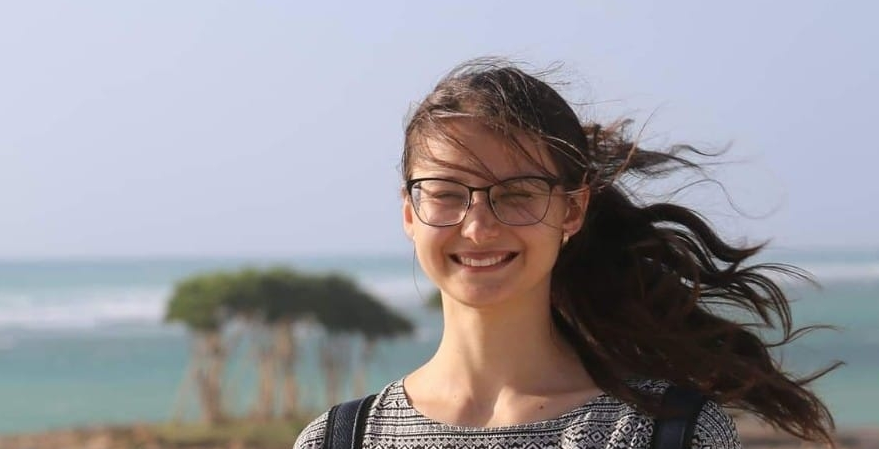
\includegraphics[height =23mm]{figures/myphoto.png}
\end{center}}
\headerbox{Motivation and introduction}{name=abstract,column=1,row=0, span=2}{
\small{Superconducting quantum circuit is one of the most robust ways for realization of quantum systems.  Observation of single photons interactions is a very interesting effect that is realized in this circuit\cite{lang2013correlations}. To conduct these experiments different devices for example, a single-photon source and a beam splitter (an element for entanglement generation) are required. For single photon experiments commercial components (photon sources, a beam splitter, detectors)  are not suitable because of dispassion  in connectors and wires. Therefore, it is natural to realize it on-chip.\\
Or another hand, conventional beam splitter has quite small bandwidth and it is not so convenient to use it. Consequently, this wide-band component on chip is interesting.}
}
%----------------------------------------------------------------------------------------
%	OTHER INSTRUMENTATION
%----------------------------------------------------------------------------------------

\headerbox{Beam splitter: the device}{name=schemebs,column=0,row=1,below=abstract2}
{\small{A hybrid microwave beam splitter (BS) consists of two branch sets, their length determine the central frequency: length = $\lambda_c/4$. To yield equal splitting 50:50 characteristic impedances have to be set as shown in Fig.1, where $Z_0=50$Ohm. For proper grounding of central polygon airbridges\cite{chen2014fabrication} are required. }
\begin{center}
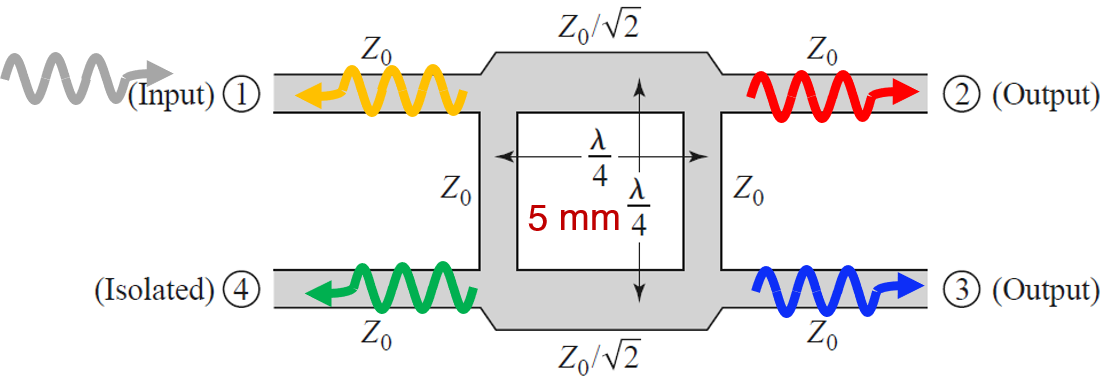
\includegraphics [height=18mm]{figures/scheme.png}
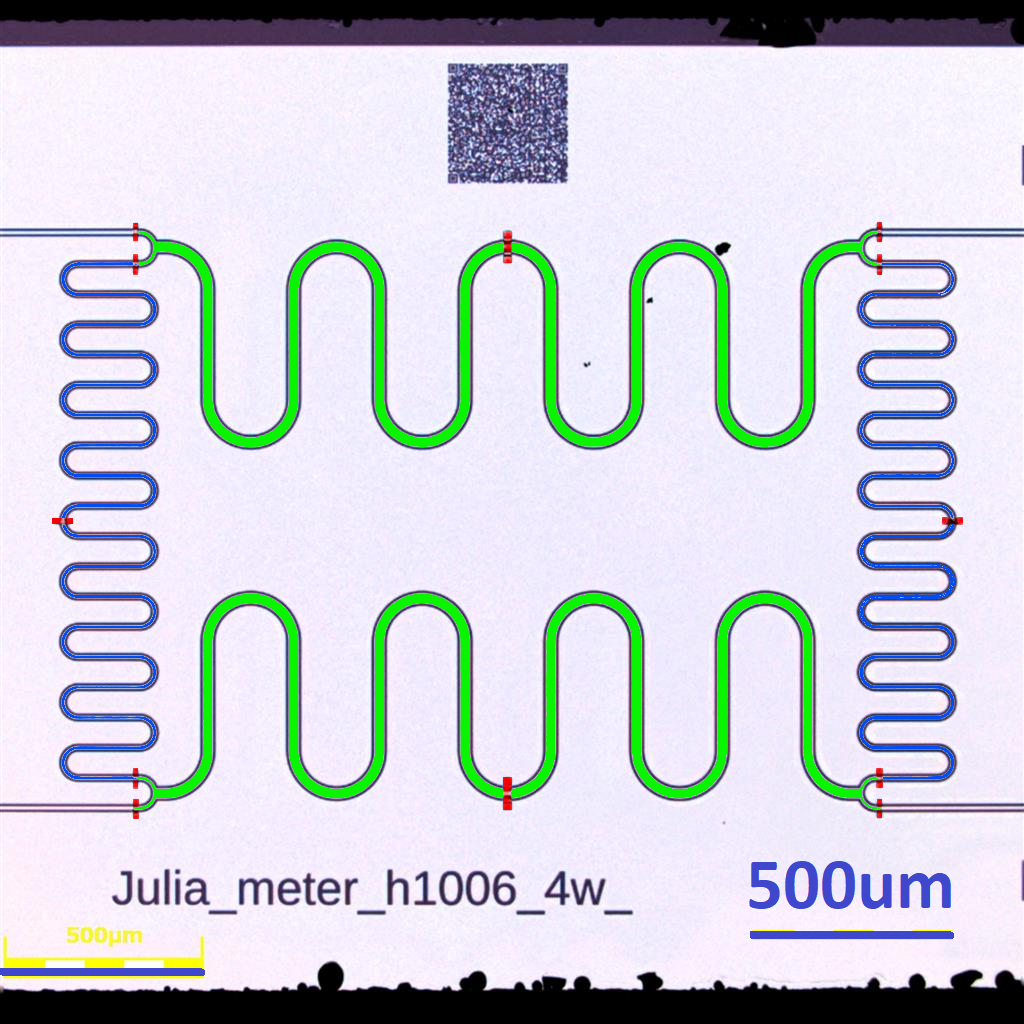
\includegraphics [height=18mm] {figures/colour2.png}
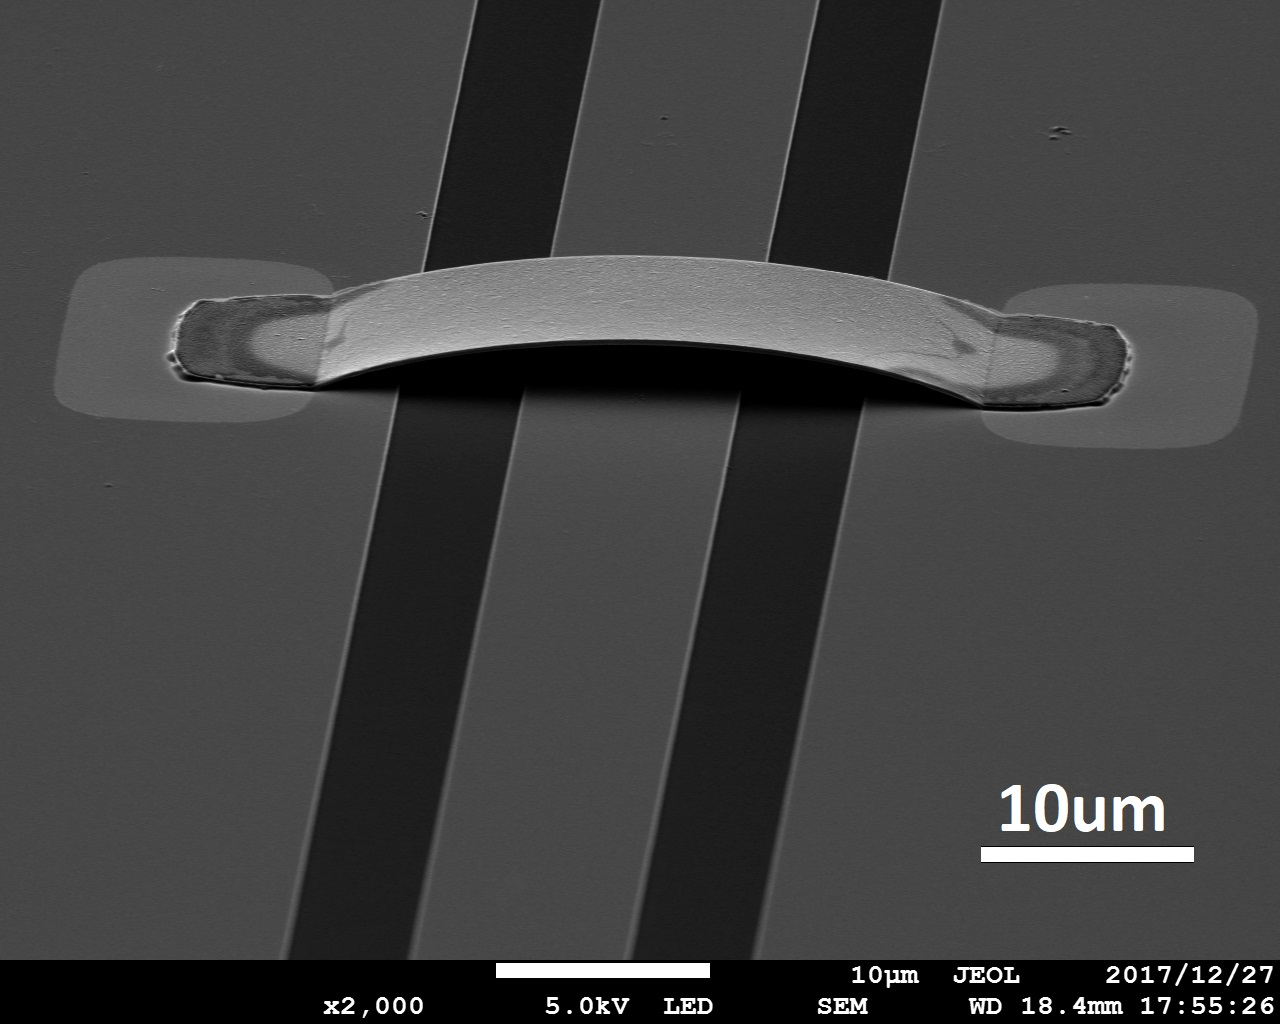
\includegraphics [height=18mm] {figures/bridge.jpg}
\end{center}
\small{\textbf{Figure 1.} Top: A scheme of beam splitter. Bottom left: fabricated beam splitter. Bottom right: a suspended airbridge.}
\begin{center}
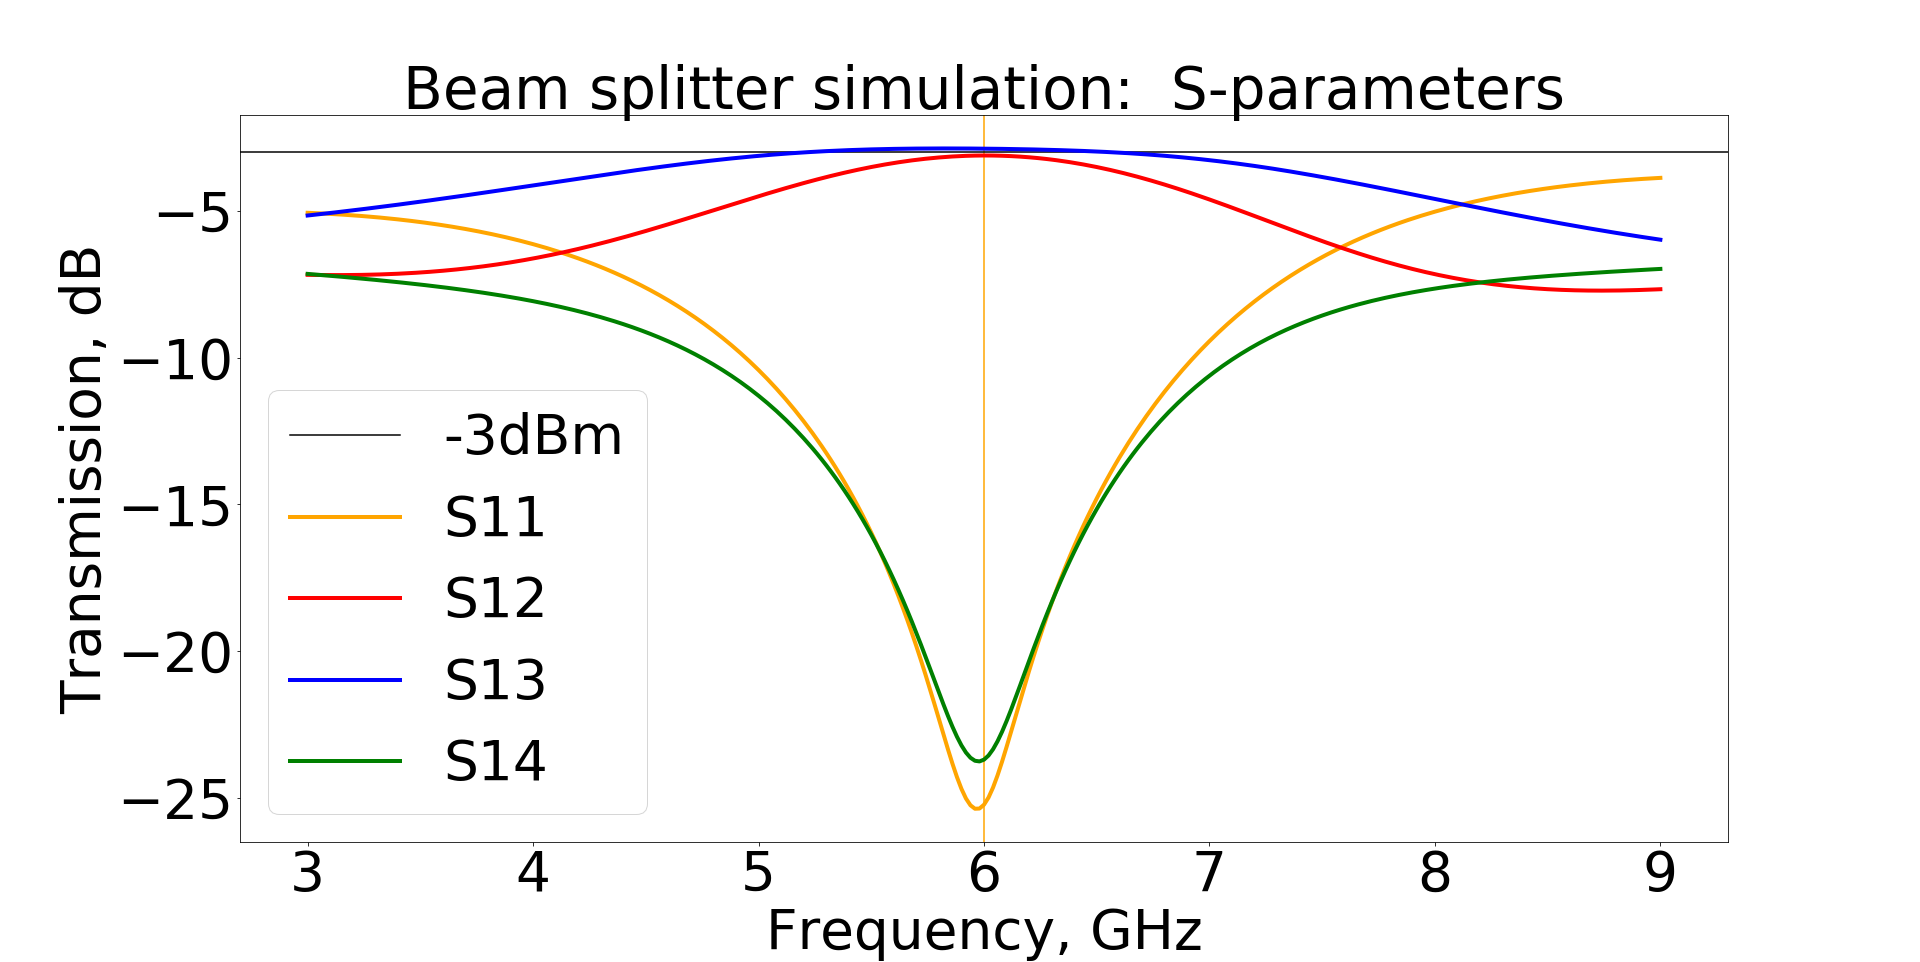
\includegraphics [height=27.5mm]{figures/simul1.png}
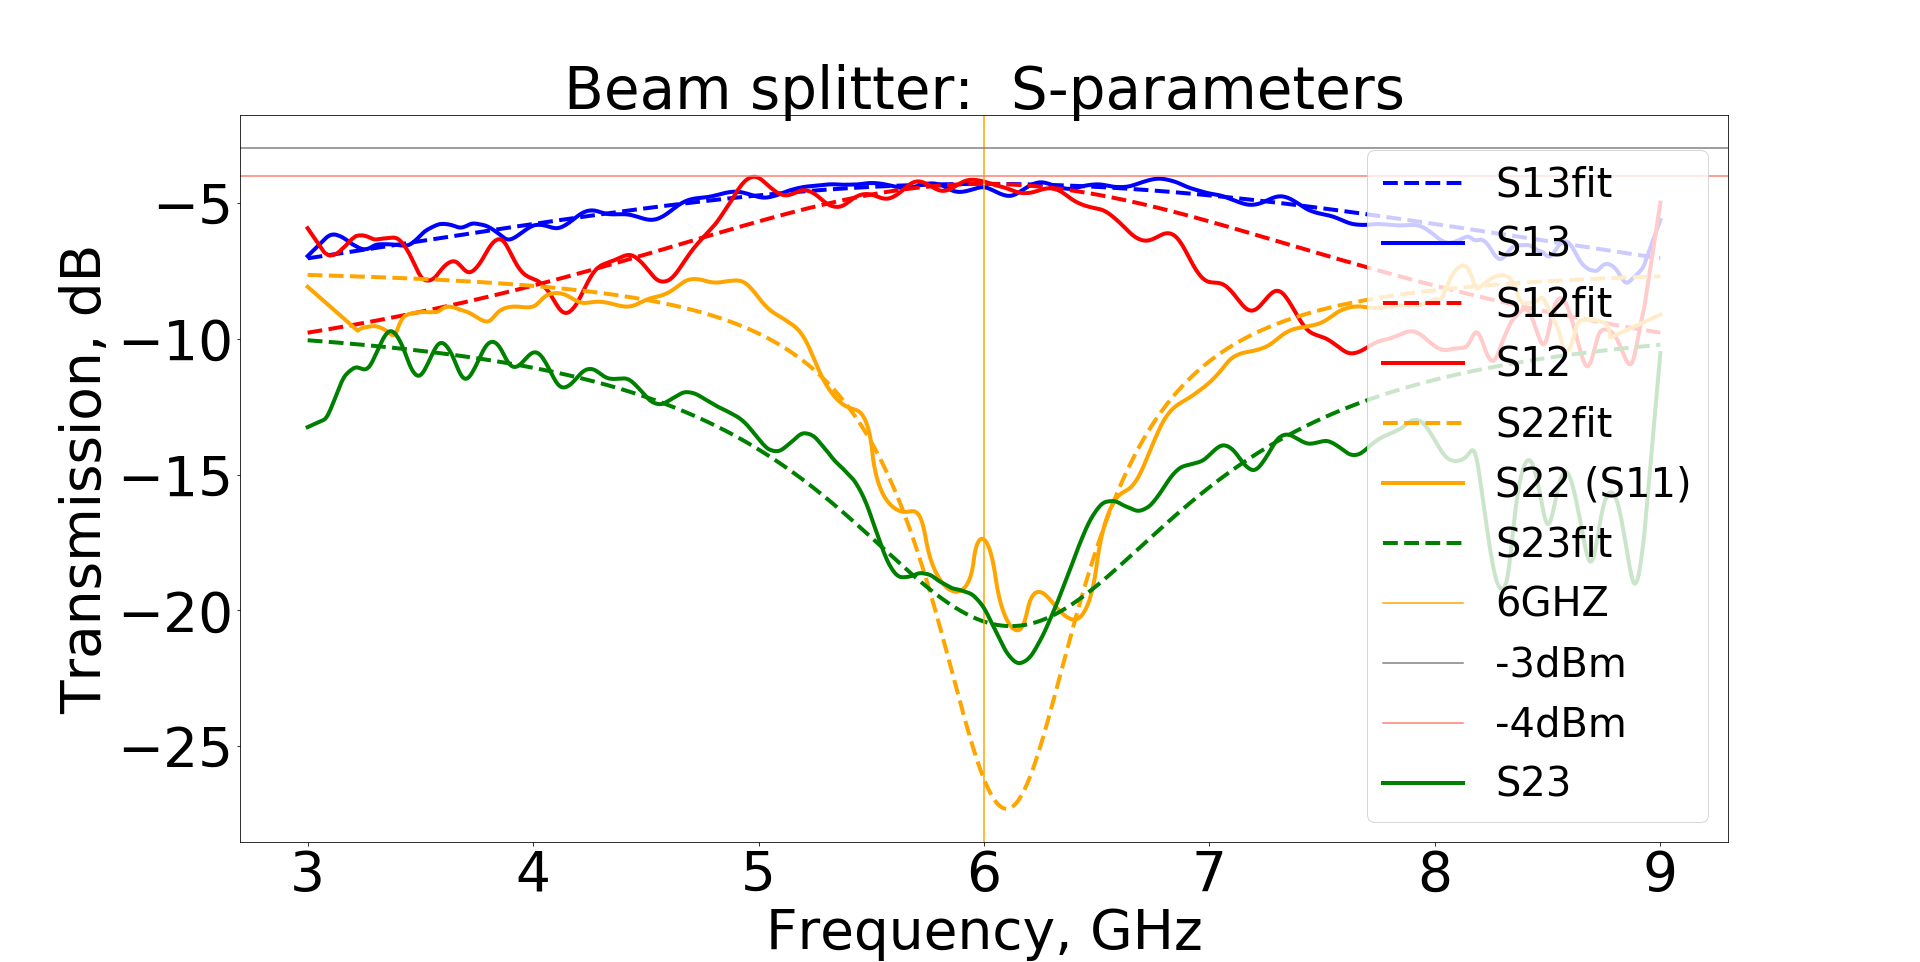
\includegraphics [height=27.5mm] {figures/4_2.png}
\end{center}
\small{\textbf{Figure 2.} S-parameters of the beam splitter. Left: Simulation. Right: Measurement at cryogenic temperature.}

}

%----------------------------------------------------------------------------------------
%	MIXER vs. SAMPLERS
%----------------------------------------------------------------------------------------
\headerbox{Scheme of wide-band double-line beam splitter}{name=scheme,span=2,column=1,row=1, below=abstract}{
\centering
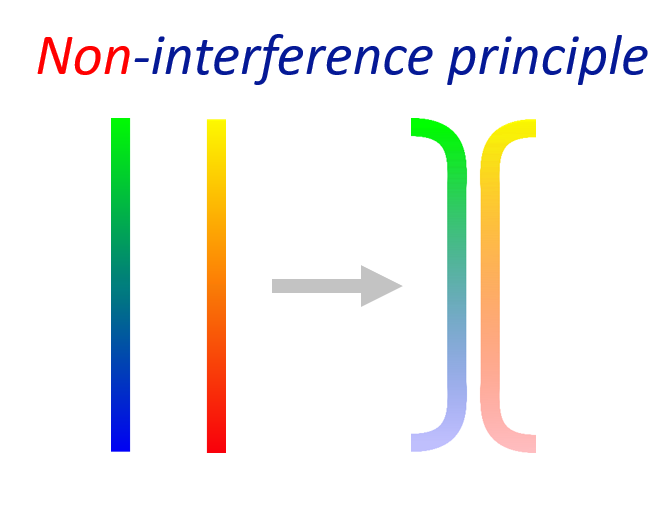
\includegraphics [height=27.53mm] {figures/ind22.png}
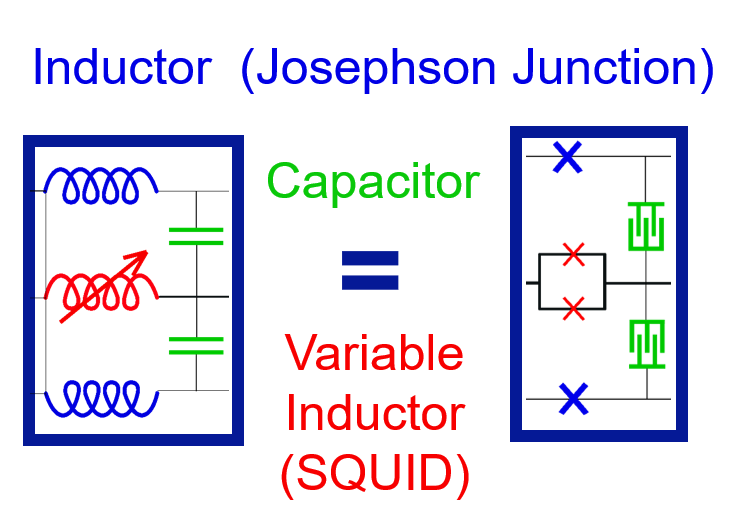
\includegraphics [height=27.53mm] {figures/ind1.png}
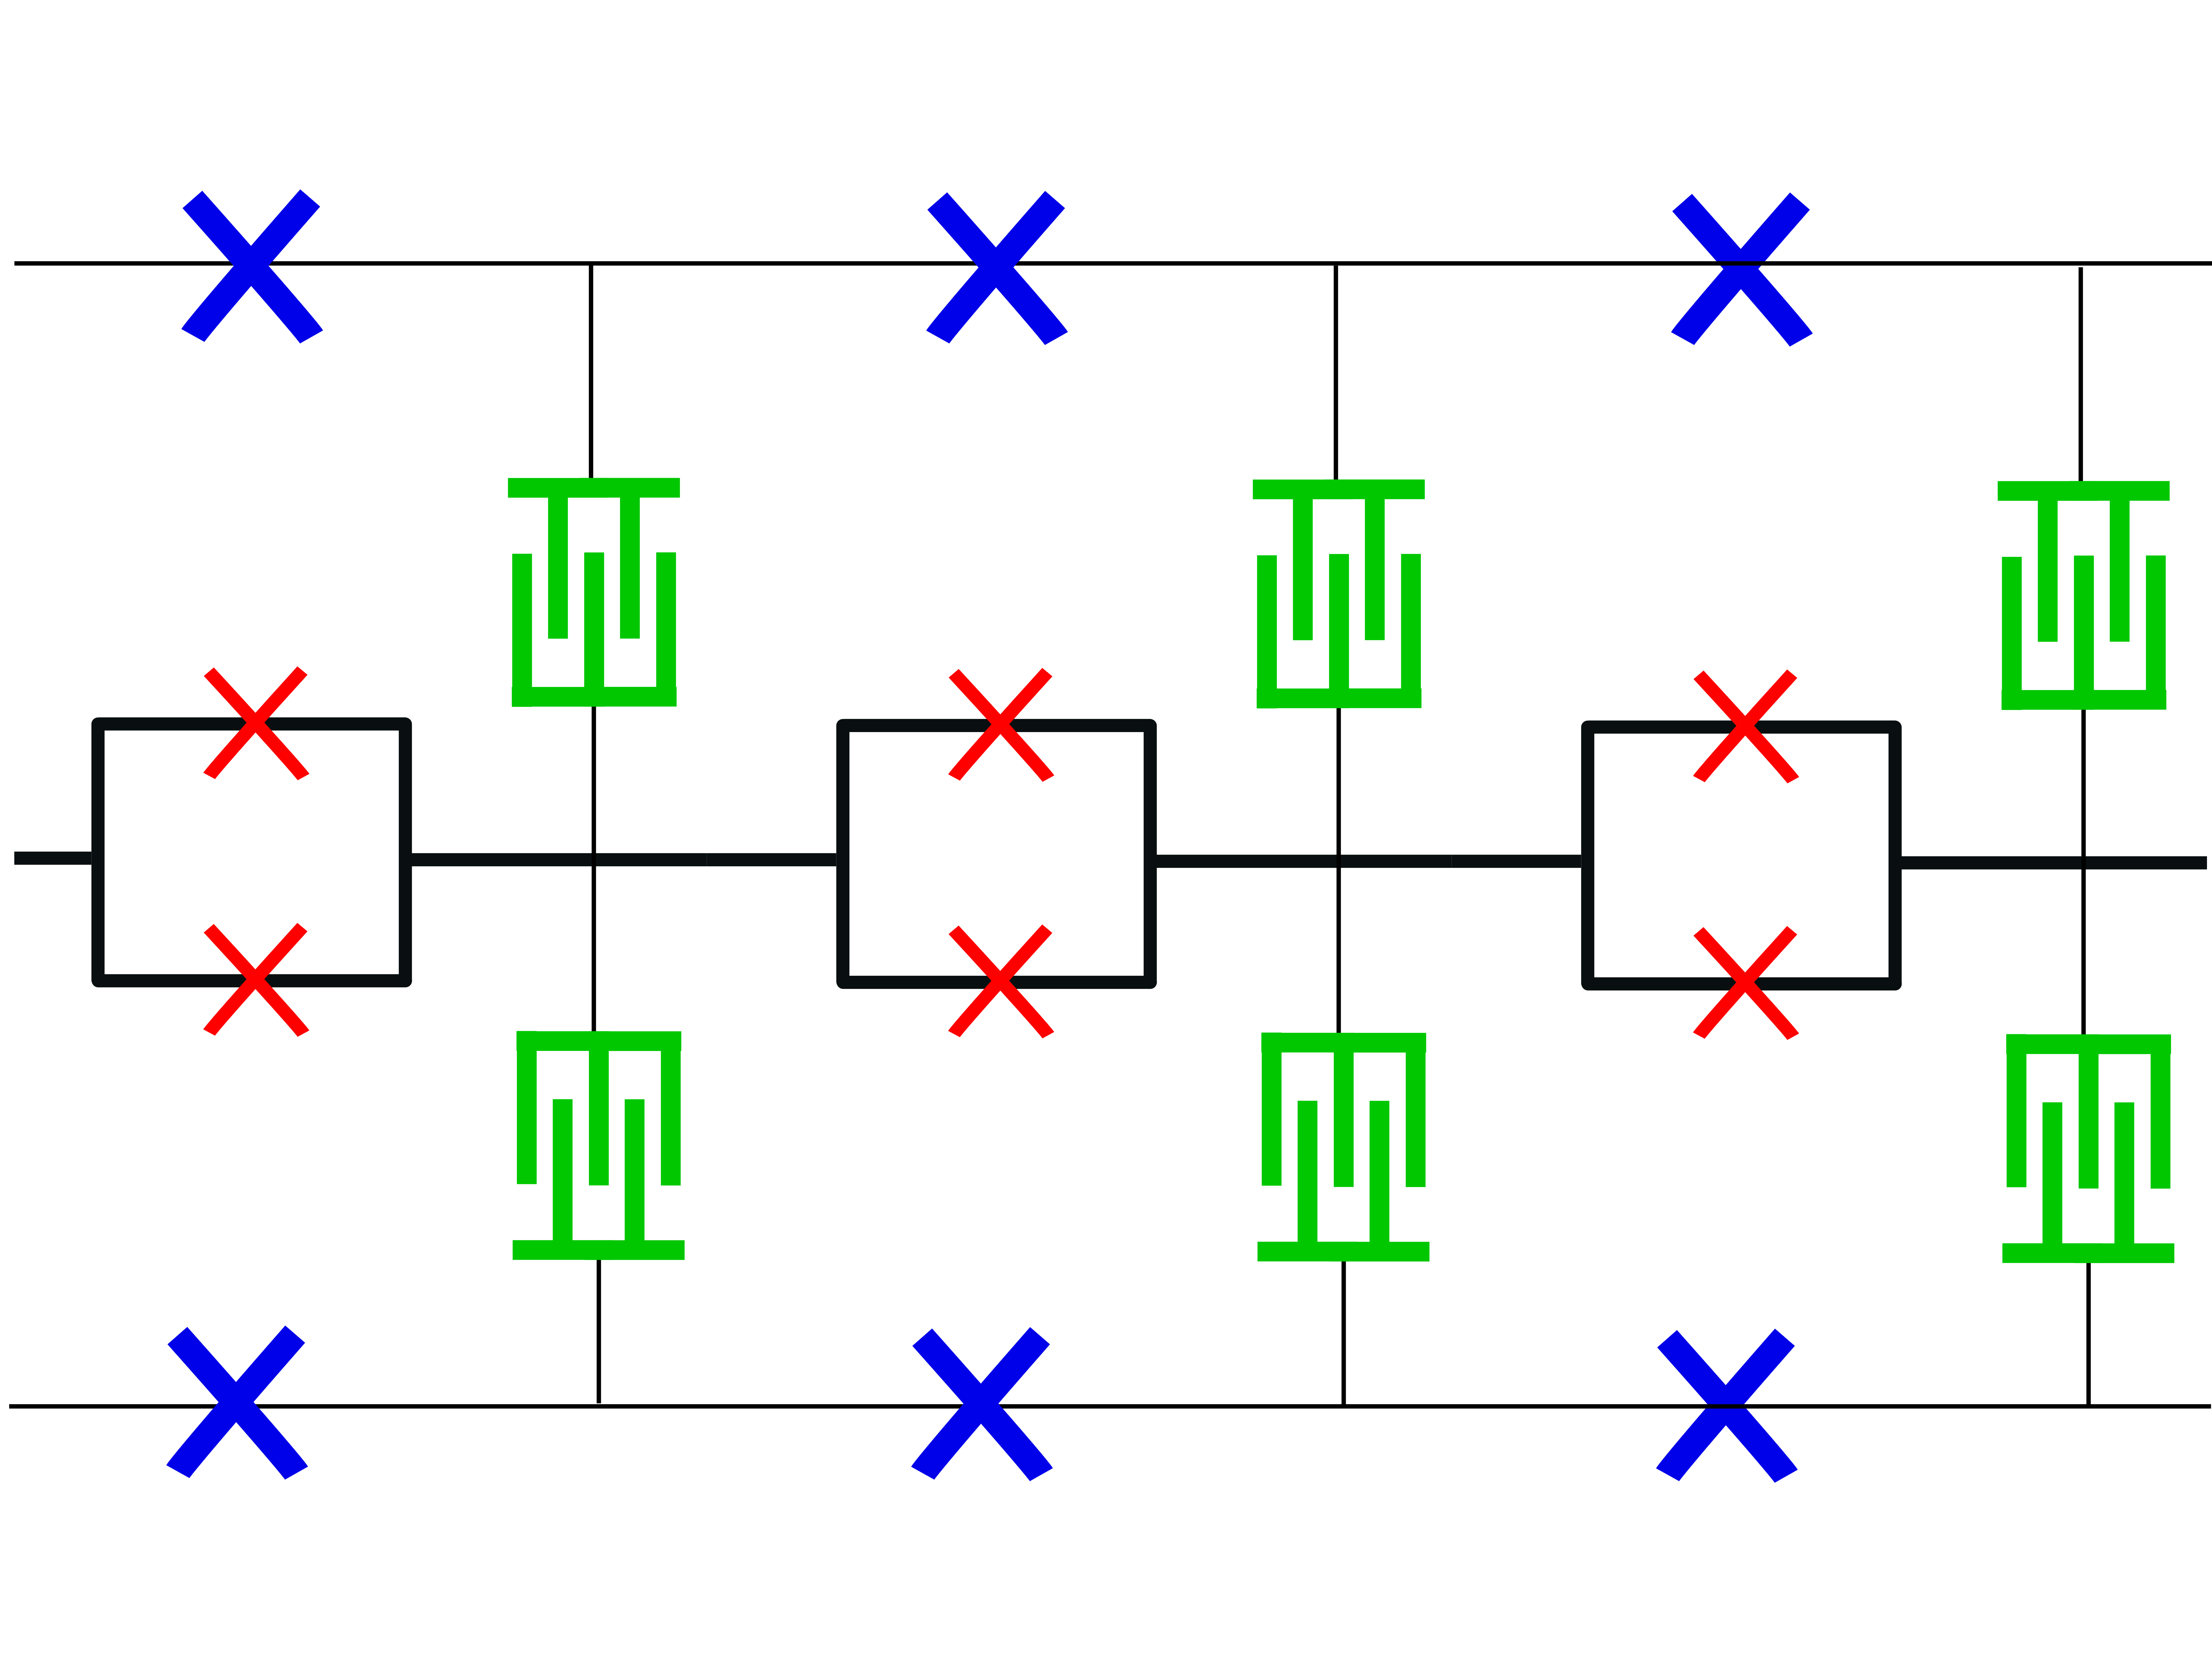
\includegraphics [height=24.5mm] {figures/single_cascade3.png}
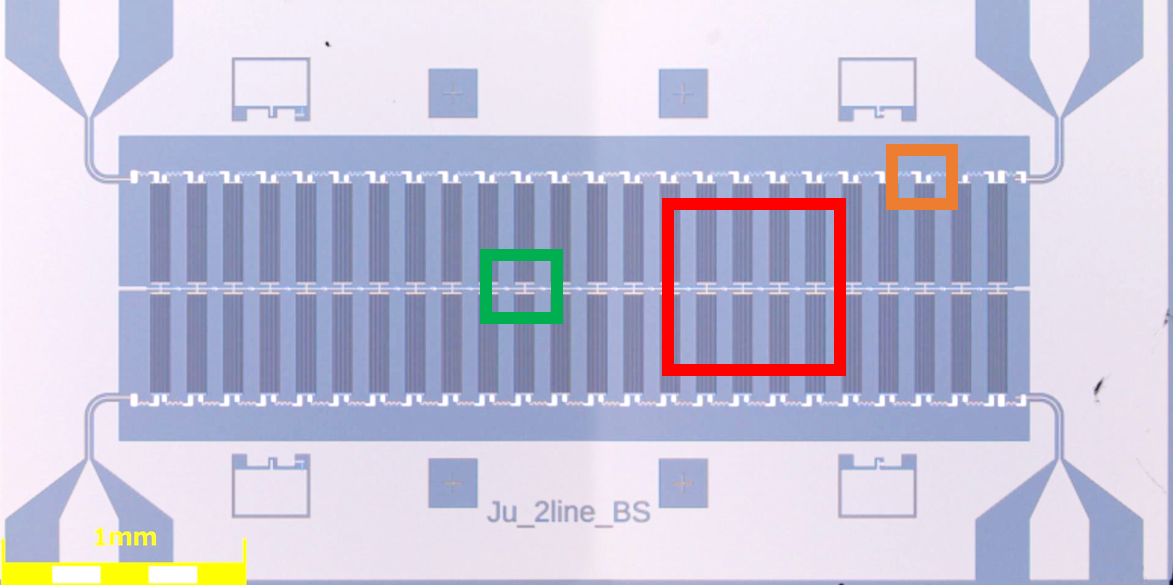
\includegraphics [height=26mm] {figures/chip1.png}
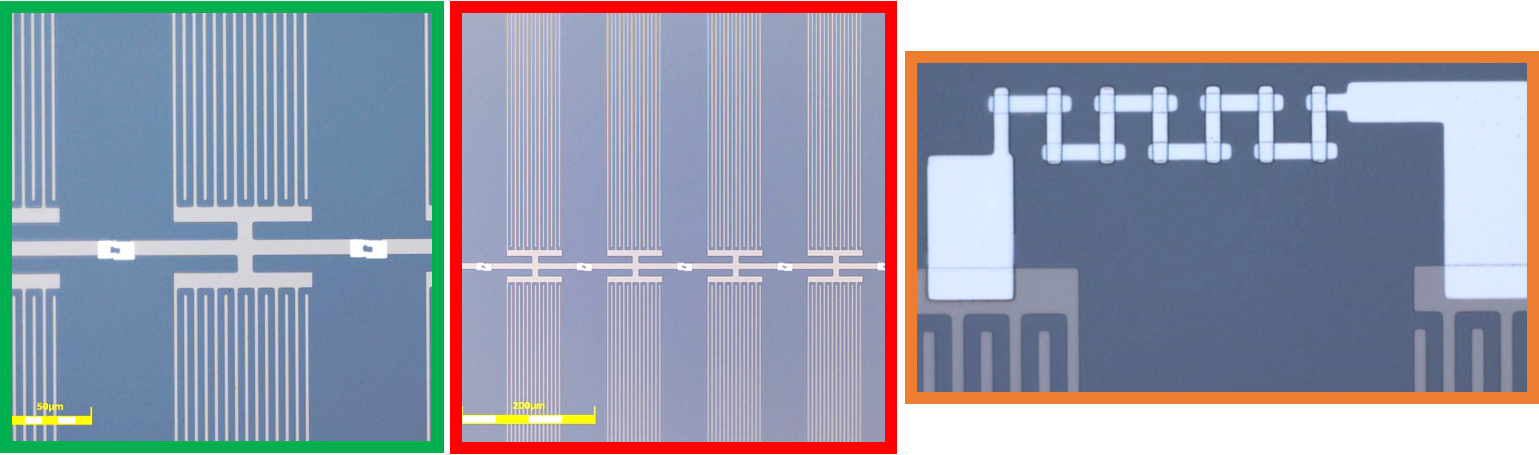
\includegraphics [height=26mm] {figures/chip2.png}\\
\textbf{Figure 3.} Top: Lamp-element scheme of the new beam splitter type. $L_{50} = 0.691 nH, C_{50} = 0.276 pF$. For $L_{coupl}$ see below. There are total 26 cascades. For equal splitting the cascade numbers is determined by \boldmath$N =\frac{1}{4(\sqrt{1+2\textcolor{red}{M}/\textcolor{blue}{L}}-1)\sqrt{\textcolor{blue}{L}\textcolor{green}{C}}f}$. Bottom: fabricated chip with this architecture.
}

\headerbox{Response and tunability}{name=restun,span=2,column=1,row=1, below=scheme}{
\centering

\includegraphics [height=20mm] {figures/picsplitting1.png}
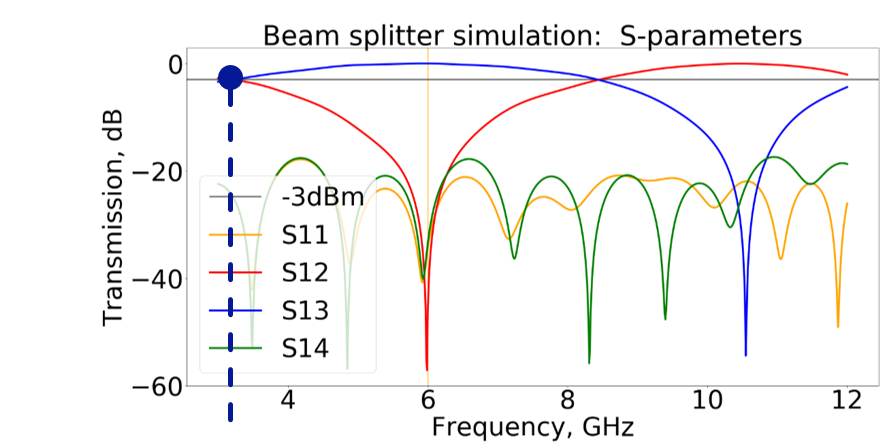
\includegraphics [height=21mm] {figures/tun1.png}
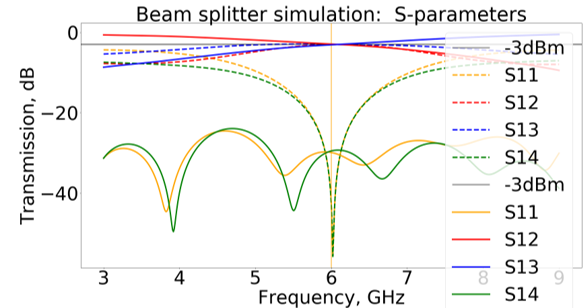
\includegraphics [height=21mm] {figures/S-par.png}
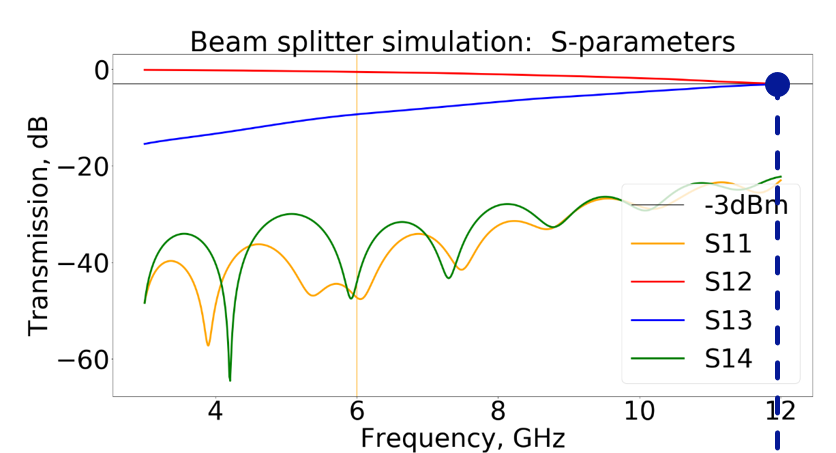
\includegraphics [height=21mm] {figures/tun2.png}\\
\textbf{Figure 4.} Simulated S-parameters of the 2line beamsplitter. Center: response of the BS on 6 GHz, $L_{coupl} = 0.09nH$ and comparison with conventional one. Left and right: S-parameters with working frequency at 3GHz (left), $L_{coupl} = 0.195nH$ and 12 GHz (Right), $L_{coupl}=0.06nH$.
}

\headerbox{Tunable microwave switch}{name=switcher,span=2,column=1,row=1, below=restun}{
\centering

\includegraphics [height=8mm] {figures/picswitch22.png}

\includegraphics [height=8mm] {figures/picswitch11.png}

\includegraphics [height=8mm] {figures/picswitch11.png}\\
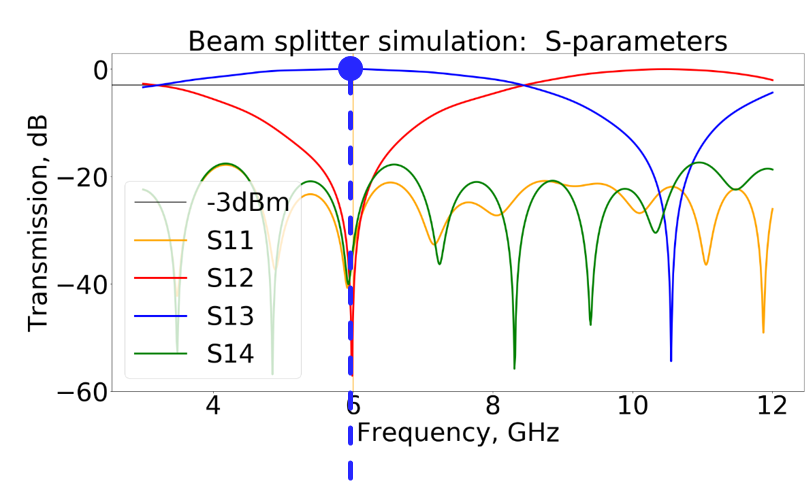
\includegraphics [height=22mm] {figures/switch1.png}
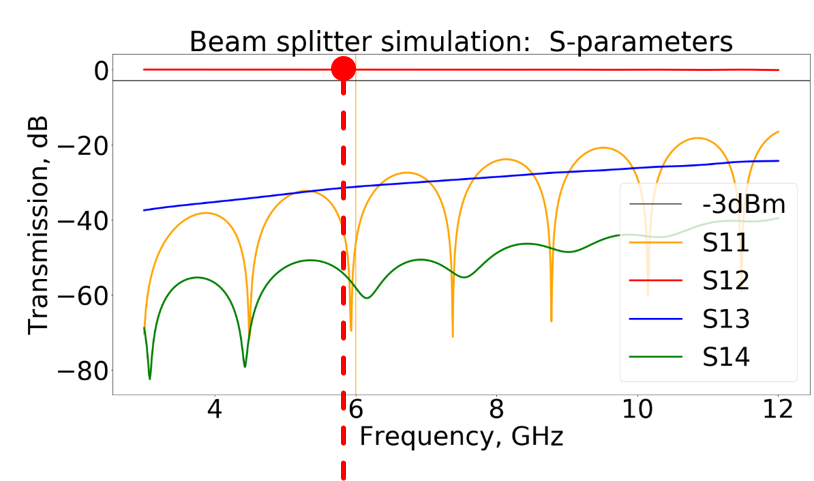
\includegraphics [height=22mm] {figures/switch2.png}
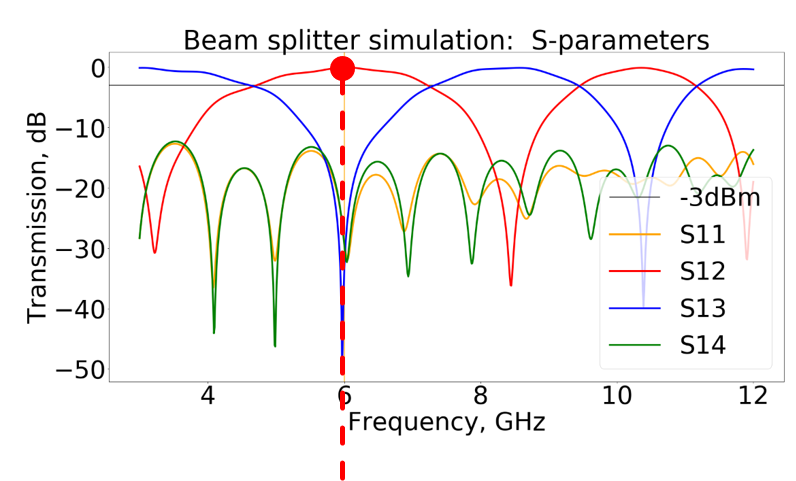
\includegraphics [height=22mm] {figures/switch3.png}\\
\textbf{Figure 5.} The switching regime. Left: the transmission only through blue output, $L_{coupl} = 0.195nH$, right: only through red channel, $L_{coupl} = 0.003nH$ and $L_{coupl} = 0.42nH$. 
}


%----------------------------------------------------------------------------------------
%	REFERENCES
%----------------------------------------------------------------------------------------
%\headerbox{References}{name=references,column=1,below=conclusion,span=2}{

%----------------------------------------------------------------------------------------
%	CONCLUSION
%----------------------------------------------------------------------------------------
\headerbox{Conclusion}{name=conclusion,column=0,row=1, below=schemebs}
{\small{Bla bla bla bla In this work simulation of new type of microwave beam splitter and fabricated device are shown. The measurement will be redo due to technical problems. The advantages of the double-line beam splitter are: wide-band frequency range, tunability from 3GHz to 12GHz and switch regime. Also, frequency for switching can be also tuned, in comparison with previous work\cite{pechal2016superconducting}. Another difference: the switched port is the same as transmission for beam splitter, in comparison with work\cite{pechal2016superconducting}. It became an opportunity to use the same component for splitter and switcher with tuned frequency without architecture changing.}}


%}
%----------------------------------------------------------------------------------------
%	ACKNOWLEDGEMENTS
%----------------------------------------------------------------------------------------
%\headerbox{Acknowledgements}{name=ack,column=0,row=2,below=conclusion}{\small{We would like to thank Hiroto Mukai, Ivan Khrapach and Gleb Fedorov for valuable discussions.}}
%\bibliographystyle{ugost2008}

%----------------------------------------------------------------------------------------
%	Refrence
%----------------------------------------------------------------------------------------
\headerbox{Reference}{name=reference,column=1, row=1, below=switcher,span=2}
{\small{\smaller{\smaller{\bibliographystyle{plain}

\bibliography{biblio}}}}}
%\headerbox{\smaller{Okinawa School in Physics 2018: Coherent Quantum Dynamics, 25 September - 4 October, Japan}}{name=conf,column=0, below=switcher,span=3}

\end{poster}
\end{document}

